\documentclass[11pt,a4paper]{article}
\usepackage{graphicx}
\usepackage{hyperref} 
\author{Akshay Deodhar - 111703013}
\title{Dynamic Programming for Sequence Alignment}
\date{}
\begin{document}
\maketitle

\section{Introduction}
The ``Central Dogma'' of molecular biology is thus- DNA is transcribed to RNA which is translated to proteins. A major problem of molecular biology is the correlation of genotype to phenotype. The genotype, of course is the base sequence in the DNA. The properties of the organism itself- such as size, shape, or ability could be considered as the phenotype. At a lower level, the function performed by proteins in a cell (and thus the structure of the protein) could be considered the phenotype.

The ability to pull out the phenotype from the genotype would mean `solving' biology. The field, however is not advanced enough to completely simulate the creation of the organism from it's DNA. Instead, common properties in different organisms are analysed to find co-relations between the genotype and phenotype. Biology is also interested in finding evolutionary relationships between organisms. 

A major problem in molecular biology is the analysis of structure and function of protein. The ability to predict structure from a protein's amino acid sequence will be world-changing.

Aligning nucleotide or amino-acid sequences to find regions of similarity will indicate correlation of common structural, functional and evolutionary properties to that region. This will provide insights into the genotype-phenotype relationship. Following Sagner's sequencing of Insulin in the 1950s, the sequencing and analysis of nucleotides and proteins has become a major field in biology. Advancements in computers have facilitated this process. Huge databases of both kinds of sequences exist and are widely used.

\section{Principle}
The computational problem to be solved in sequence alignment is thus: \begin{quote}What is the best possible way these to match these sequences ? \end{quote}Consider the sequences \emph{ATGCATT} and \emph{TTGC}. By observation, we could say that the second `T' of the second sequence should be aligned with the first `T' in the first sequence. But strings are much more complex and `common sense' solution does not suffice in science. Using programs to perform this task makes it structured, accurate and fast. There are several cases of the problem, such as \emph{pairwise alignment, multiple sequence alignment, global alignment and local alignment}.

	Sequence matching programs with definitions of what constitutes the \emph{best possible alignment} for the particular pair of strings are used for this purpose. This is done by deciding a \emph{cost function} for particular mutations such as deletion, insertion or replacement of a base in a sequence. More likely mutations are prescribed with a lower cost, whereas unlikely ones are prescribed a higher cost.Thus, for a particular way to match the two strings, a total cost can be calculated. The problem can now be reframed formally as:\begin{quote} Minimize the cost of matching the sequences $A$ and $B$ consisting of $m$ and $n$ bases respectively given $costfunction(operation, base1, base2)$ \end{quote} This cost is determined empirically using statistical biological observations. With a more `mathematical' formulation of the problem, dynamic programming comes into play.

		\section{Method}

Now, a brute-force method to solve this would be to calculate the cost for all possible matches, and chose the one for which it is minimum. But such an algorithm would be computationally expensive with a complexity of \emph{n X m} for sequences of length \emph{m} and \emph{n} respectively.

An alternate way to think about the problem would be finding \emph{the minimum number of changes required to convert one string to another}. For example, in the above quoted example, aligning `TT' to `TT' would mean that `ATGCA' in the first string would be deleted, and the sequence `GC' would be appended to obtain the second. This approach and the use of \emph{``dynamic programming''}\footnote{Actually, there is nothing `dynamic' about dynamic programming. It just happened that it's inventor, Richard Bellman was working for a company with a U.S military contract. The military had a notorious hatred of math, and Bellman simply created a fancy name to impress the bigwigs and keep his work going} can provide an optimal solution.

Dynamic Programming is computer programming method which breaks a big problem into several smaller sub-problems, and stores the solution of a solved sub-problem for future use. This storage of results prevents excess computation, as the answers for already solved-for cases be looked up rather than be solved for again.

The dynamic programming approach to solve the alignment problem involves finding the sequence of edits with the minimum `mutation' cost. The sequences are considered as strings $A[1 .... m]$ and $B[1.... n]$ of bases (or amino acids). The string $A$ is to be converted to $B$ in  a sequence of steps. At each step, there are three possible choices
\flushleft
\vbox{%
	\begin{enumerate}
		\item \emph{Insert the first character of substring B}
		\item \emph{Delete the first character of substring A}
		\item \emph{Replace the first character of A with the first character of substring B}
	\end{enumerate}
	\cite{dp}}

	Each choice will have it's associated cost. Thus the minimum cost for the matching at a particular step will be given as

	\begin{center}$mincost(A[1.. i], B[1.. j]) = mincost(A[1], B[1]) + mincost(A[2... i], B[2.. j])$\end{center}\footnote{the subarray A[x... y] itself will be considered as an \emph{array} in the called function. Thus, in the next function call, A[1] will actually be A[x], and so on}

		Where $mincost(A[],B[])$ is the minimum cost of matching those particular parts of strings $A$ and $B$

	Now, the cost of matching nothing to nothing is 0. This can be used as the base case to formulate this problem in terms of a cost matrix $cost[m][n]$, where the cell $cost[i][j]$ represents the cost of matching \emph{A[1.. i]} to \emph{B[1.. j]}. Thus, the bottom right corner $cost[m][n]$ represents the minimum cost of matching \emph{A} and \emph{B}. The top-left corner represents the cost of matching nothing to nothing, which is zero. Using this as out `root-case' we can fill up matrix to obtain the value of $cost[m][n]$
	The cost at $cost[i][j]$ is given as:

	\begin{center}cost[i][j] = min(cost[i - 1][j] + delete(A[i]),\\
		cost[i][j - 1] + insert(B[j]),\\
					cost[i - 1][j - 1] + replace(A[i], B[j])\footnote{the expression for value in cell is different for cells at the edges and corners}

	\end{center}
			Where the $delete(), insert()$ and $replace(,)$ functions give the corresponding costs\cite{cs50} The algorithm goes on to populate the matrix row by row, to finally yield the optimized solution in the cell $cost[m][n]$. The dynamic programming approach for edit distance has a time complexity of $O(mn)$ (a significant improvement over the brute force method).
				\begin{figure}
					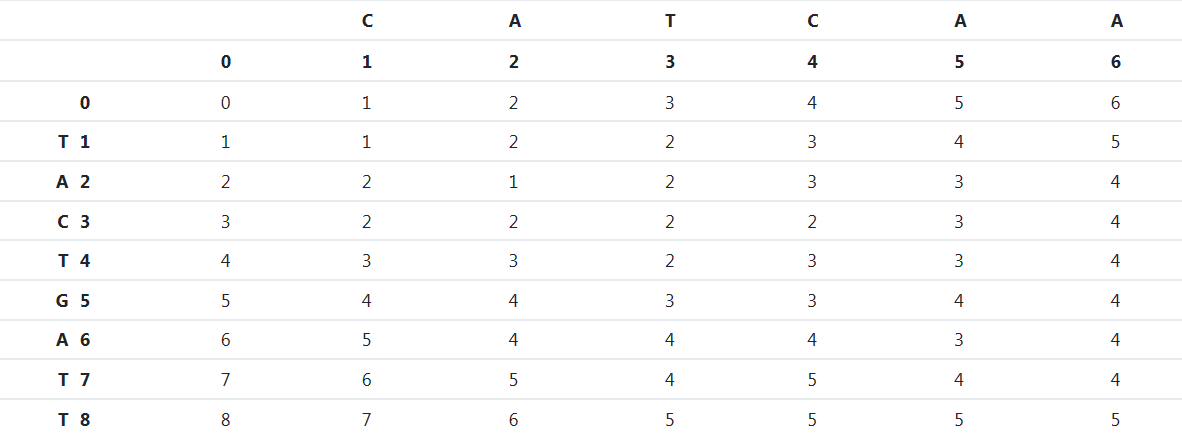
\includegraphics[width=\linewidth]{dpcost.png}
					\caption{Cost Matrix. Moving downward represents a deletion, moving diagonally represents a replacement (replacing by same base has zero cost), and moving right represents an insertion\cite{costmat}}
					\label{fig:costmatrix}
				\end{figure}

				\section{Application}

				The explanation given above is a simplified explanation. Variants of this method such as the \emph{Smith Waterman} algorithm and \emph{Needleman Wunsch} algorithm are used in actual scenarios. Such dynamic programming algorithms are guaranteed to find the optimal solution for a given cost function. But they are computationally expensive. 


				Modern algorithms which give fast approximations like those used in \emph{BLAST} or \emph{FASTA} programs have developed, which are used for sequence database search. Several other programs- multiple sequence alignment programs like \emph{CLUSTALW}, profile search programs like \emph{HMMER}, gene finding programs like \emph{GENSCAN} are based on dynamic programming.\cite{arti}

				Sequence alignment of nucleotides can yield information about functional and evolutionary similarities. If two sequences which show significant alignment are known to share a common ancestor, mismatches and blanks could be interpreted as mutations which were introduced in one or both lineages
				when they diverged during evolution. In sequence alignment of proteins, similarity in amino acids occupying a particular position in the proteins will point to that region being \emph{`conserved'} or being a part of a \emph{`sequence motif'}. This means that that particular region has remained unchanged during evolution, and thus has is important to organisms. Such a sequence is said to be \emph{biologically significant}. 

				\begin{thebibliography}{99}
					\bibitem{costmat}\url{http://similarities.cs50.net/more}
					\bibitem{arti}\url{http://www.genebio.ufba.br/wp-content/uploads/dynamic_programming.pdf}
					\bibitem{wikipedia}\url{https://en.wikipedia.org/wiki/Sequence_alignment}
					\bibitem{dp}\url{https://en.wikipedia.org/wiki/Dynamic_programming}
					\bibitem{cs50}\url{https://docs.cs50.net/2017/fall/notes/7/lecture7.html}
					\bibitem{geb}Godel, Eshler, Bach: An Eternal Golden Braid, \emph{Douglas Hofstader}
				\end{thebibliography}


			\end{document}

